Escribe una expresión para calcular el perímetro y el área de la figura \ref{fig:20230319044552}

\begin{figure}[H]
    \centering
    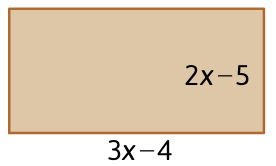
\includegraphics[width=0.25\textwidth]{../images/20230319044552}
    \caption{}
    \label{fig:20230319044552}
\end{figure}

\begin{solutionbox}{3.5cm}
    \begin{multicols}{2}
      Perímetro:
      \begin{align*}
        P & =2(3x-4)+2(2x-5) \\
          & =6x-8+4x-10      \\
          & =10x-18
      \end{align*}
    
      Área:
      \begin{align*}
        A & =(3x-4)(2x-5)     \\
          & =6x^2-15x-8x+20  \\
          & =6x^2-23x+20
      \end{align*}
    \end{multicols}
  \end{solutionbox}
